\documentclass{beamer}
\usetheme{Ilmenau}
\setbeamercovered{transparent}
%\setbeamercovered{invisible}
\setbeamercolor*{item}{fg=blue}

\usepackage{caption}
\captionsetup{font=scriptsize,labelfont=scriptsize}
\usepackage{hyperref}
\hypersetup{urlcolor=blue}
\usepackage[utf8]{inputenc}
\usepackage[T1]{fontenc}
\usepackage[ngerman]{babel}

\title{DNA - Computing}
\author{Aleyna Acikyol \& Alina Grahic}
\date{29. Oktober 2021}

\begin{document}
\begin{frame}[plain]
    \maketitle
\end{frame}
%2
\begin{frame}{Inhalt}
	\begin{itemize}
	\item Einleitung: Probleme heutiger Computer
	\pause	
	\item Crash-Kurs: DNA
	\pause
	\item DNA-Computing	
	\begin{itemize}
		\item 	Was ist das?
		\item Warum DNA?	
	\end{itemize}
	\pause
	\item Vor- und Nachteile
	\pause
	\item Quellen
\end{itemize}
\end{frame}

%3 FOTO
\begin{frame}{Probleme heutiger Computer (1)}
	\begin{itemize}
	\item	Datenträger
	\end{itemize}

\begin{figure}	
	%\begin{itemize}
		\begin{columns}
			\column{0.50\linewidth}
			\centering
			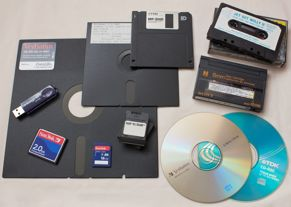
\includegraphics[height=3cm, width=4cm]{./3.jpg}\caption{[2]diverse Datenträger im Privatgebrauch, wikipedia}
			
			\column{0.50\linewidth}		
			\centering
			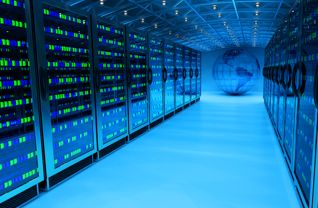
\includegraphics[height=3cm, width=4cm]{./3.2.jpg}\caption{[3]Data Centre, Cloud}
		\end{columns} 
	%\end{itemize}
\end{figure}
\end{frame}

%4
\begin{frame}{Probleme heutiger Computer (2)}
	\begin{enumerate}
	
	\item \textcolor{blue}{Datenspeicher:}
	\begin{itemize}
		\item 	Inschriften, Bücher, Festplatten, CDs, …
		\item immer mehr Daten zu speichern
	\end{itemize}
\pause
	\item \textcolor{blue}{Auf Dauer mit konventionellen Methoden schwierig:}
	\begin{itemize}
		\item 	Haltbarkeit von Speichergeräten
		\item Platz und Ressourcen
		
	\end{itemize}

	\end{enumerate}
\end{frame}

%5 FOTO
\begin{frame}{Probleme heutiger Computer (3)}
	%\begin{enumerate}
	%	\item \textcolor{blue}{Transistoren:}
		\begin{itemize}
			\item \textcolor{blue}{Transistoren:}
			\begin{itemize}
				\item kleiner geht nicht
			    \item Ausgleich mit Multicores /Multiprozessorsysteme
			\end{itemize}
		\end{itemize}
		%\pause
	
\begin{figure}	
	%\begin{itemize}
	\begin{columns}
		\column{0.50\linewidth}
		\centering
		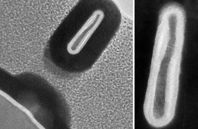
\includegraphics[height=3cm, width=3cm]{./5.jpg}\caption{[4]3D Transistor mit 2,5nm Durchmesser, newatlas.com}
		
		\column{0.50\linewidth}		
		\centering
		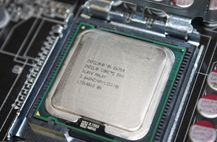
\includegraphics[height=3cm, width=3cm]{./5.2.jpg}\caption{[5] Ein Intel Core 2 Duo E6750 dual-core Prozessor, wikipedia.org}
	\end{columns} 
	%\end{itemize}
\end{figure}
	%\end{enumerate}	
\end{frame}

%6 FOTO
\begin{frame}{DNA (1)}
	\begin{itemize}
		\begin{columns}
			\column{0.50\linewidth}
			\centering
			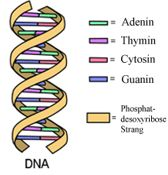
\includegraphics[height=4cm, width=4cm]{./6.jpg}%\caption{Aufbau DNA}
			\captionof{figure}{[6]Aufbau DNA}%
			
			\column{0.50\linewidth}		
				\item Desoxyribonukleinsäure
			\pause \item Speicherung der Erbinformationen/ Multiprozessorsysteme
			\pause \item Doppelhelix 
			\pause \item Grundbausteinen:   
				\begin{itemize}
				\item kleiner organische Basen
				\item Zuckermoleküle
				\item Phosphatgruppen  
			 \end{itemize} 
		\end{columns} 
	\end{itemize}
\end{frame}


%7 FOTO
\begin{frame}{DNA (2)}
	\begin{columns}
	\column{0.50\linewidth}
	\centering
	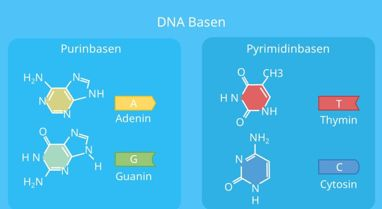
\includegraphics[height=3cm, width=5cm]{./7.jpg}%\caption{Aufbau DNA}
	\captionof{figure}{[8] Chemische Struktur der DNA Basen, studyflix.de}
		
	\column{0.50\linewidth}		
	\begin{enumerate}
	\item \textcolor{blue}{Codierung der vier Basen:}
 	\begin{itemize}
 	\item Adenin \item Cytosin
 	\item Guanin \item Thymin 
     \end{itemize} 
	\end{enumerate}

\begin{itemize}	
	\item Abfolge der Basen $\rightarrow$  genetischen Informationen festgelegt $\rightarrow$ Genetischer Code	
\end{itemize} 

\end{columns} 
\end{frame}

%8
\begin{frame}{DNA-Computing (1)}

	\begin{itemize}	
	\item 	Was ist das?
\pause	\item Hardware beruhend auf DNA, Biochemie und Molekularbiologie
\pause	\item 	Wozu DNA?
\end{itemize} 
	
\end{frame}

%9 
\begin{frame}{DNA-Computing (2)}
	\begin{enumerate}
	\item \textcolor{blue}{Verfügbarkeit:}
		\begin{itemize}	
		\item Materialien zur Herstellung von DNA fast überall zu finden
	\end{itemize} 
\pause \item \textcolor{blue}{Lange Haltbarkeit:}
\begin{itemize}	
	\item 1000 + Jahre unter bestimmten Bedingungen
\end{itemize} 
\pause \item \textcolor{blue}{Umweltfreundlich:}
\begin{itemize}	
	\item  Natürliche Moleküle verwendet ugiftig recyclebar  	
\end{itemize} 
	\end{enumerate}
\end{frame}

%10
\begin{frame}{DNA-Computing (3)}
	\begin{enumerate}
		\item \textcolor{blue}{Parallelisierung:}
		\begin{itemize}	
			\item Jeder Strang entspricht einer Operation
			Mehrere Billionen Stränge in einem Reagenzglas 
		\end{itemize} 
		\item \textcolor{blue}{Enorme Speicherkapazität:}
		\begin{itemize}	
			\item 10 Billionen (1012) DNA Stränge in 1 	${cm}^3$ d.h. $\sim$ 10Terabyte an Daten
			Bzw. 1 Gramm DNA $\sim$ 455 Exabyte
		\end{itemize} 
	\end{enumerate}
\end{frame}

%11
\begin{frame}{Vor - und Nachteile}
	\begin{itemize}
	\item sehr langsam Antworten 
	\pause \item lange Lese- und Schreibgeschwindigkeit 
	\pause \item Ergebnisse schwieriger zu verwerten
	\pause \item nicht besonders praxistauglich	
	\pause \item Speichereinheiten sehr klein 	
	\pause \item schnellere Beschädigung der Daten durch UV-Strahlung  	
	\pause \item längere Lebenszeit	
	\pause \item geringere Stromverbrauch	
	\pause \item erhöhte Datensicherheit 	
	\pause \item bessere Schutz vor Hackerangriffen
	\end{itemize}
\end{frame}

%12 FOTO
\begin{frame}{Anfänge}
		\begin{columns}
		\column{0.40\linewidth}
		\centering
		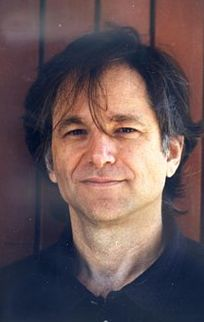
\includegraphics[height=5cm, width=4cm]{./12.jpg}%\caption{Aufbau DNA}
		\captionof{figure}{[10] Leonard Adleman, wikipedia.org}%
		
		\column{0.50\linewidth}		
		\begin{itemize}
	\item  1994 
	\pause \item  Leonard Adleman 
	\pause \item TT-100 (Testtube mit 100 Mikrolitern) 
	\pause \item Hamiltonsches Wegproblem  
		\end{itemize}
	\end{columns}
\end{frame}

%13 FOTO
\begin{frame}{Aktuellere Errungenschaften}
	\begin{itemize}
		\item Microsoft and UW demonstrate first fully automated DNA data storage
	\end{itemize}

	\begin{columns}
		\column{0.50\linewidth}
		\centering
		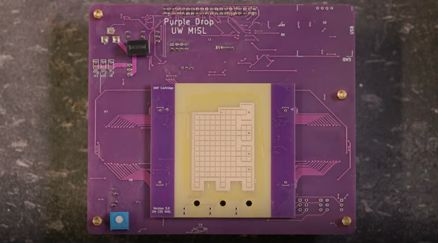
\includegraphics[height=3cm, width=5cm]{./13.jpg}%\caption{Aufbau DNA}
		\captionof{figure}{https://www.youtube.com/watch?v=60Gi5lqL-dA}
\end{columns}
\end{frame}
%14
\begin{frame}{Quellen – Abbildungen}

\begin{enumerate}
\item \href{https://de.futuroprossimo.it/2020/01/un-computer-di-dna-puo-calcolare-la-radice-quadrata-di-numeri-fino-a-900/}{https://de.futuroprossimo.it}
\item 
\href{https://pl.wikipedia.org/wiki/No\%C5\%9Bnik_danych}{https://pl.wikipedia.org}
\item
\href{https://www.titanpower.com/blog/increasing-rate-of-data-production-prompts-google-to-rethink-data-center-storage/}{https://www.titanpower.com}
\item
\href{https://newatlas.com/smallest-transistors-microfabrication/57583/}{https://newatlas.com}
\item
\href{https://en.wikipedia.org/wiki/Multi-core_processor}{https://en.wikipedia.org/wiki/Multi-core\_processor}
\item
\href{ https://internet-evoluzzer.de/mars-versus-venus-teil-5-schimpansen-mann-und-menschen-frau/}{https://internet-evoluzzer.de}
\item
\href{ https://www.lecturio.de/magazin/dna/}{https://www.lecturio.de}
\item
\href{https://studyflix.de/biologie/dna-desoxyribonukleinsaure-2444}{https://studyflix.de}
\item
\href{https://www.thieme.de/de/psychiatrie-psychotherapie-psychosomatik/sozialpsychiatrie-kann-abgeschafft-werden-pro-kontra-53872.htm}{https://www.thieme.de}
\item
\href{https://de.wikipedia.org/wiki/Leonard_Adleman}{https://de.wikipedia.org/wiki/Leonard\_Adleman}
\end{enumerate}
\end{frame}

%15
\begin{frame}{Quellen - Inhalt}
\begin{enumerate}
\item		
\href{https://www.simplyscience.ch/kids/wissen/dna-was-ist-das
}{https://www.simplyscience.ch}	
\item
\href{https://www.lecturio.de/magazin/dna/}{https://www.lecturio.de}
\item
\href{https://studyflix.de/biologie/dna-desoxyribonukleinsaure-2444}{https://studyflix.de}
\item
\href{https://de.serlo.org/biologie/70762/dna-was-ist-das}{https://de.serlo.org}
\item
\href{https://www.frustfrei-lernen.de/biologie/dna-dns-aufbau-struktur.html}{https://www.frustfrei-lernen.de}
\item
\href{https://de.wikipedia.org/wiki/DNA-Computer}{https://de.wikipedia.org/}
\item
\href{https://www.youtube.com/watch?v=qwjQcBhervk}{https://www.youtube.com/watch?v=qwjQcBhervk}
\item
\href{https://de.wikipedia.org/wiki/TT-100}{https://de.wikipedia.org/wiki/TT-100}
\item
\href{https://interestingengineering.com/what-is-dna-computing-how-does-it-work-and-why-its-such-a-big-deal}{https://interestingengineering.com}
\item
\href{https://www.virginialeenlaw.com/help/readers-ask-how-much-data-can-be-stored-in-dna.html}{https://www.virginialeenlaw.com}
\item
\href{https://www.youtube.com/watch?v=wxStlzunxCw}{https://www.youtube.com/watch?v=wxStlzunxCw}
\item
\href{https://www.youtube.com/watch?v=vefBhhjodpE}{https://www.youtube.com/watch?v=vefBhhjodpE}
\item
\href{https://www.youtube.com/watch?v=1_OMEQ5SORg&t=156s}{https://www.youtube.com/watch?v=1\_OMEQ5SORg}

\end{enumerate}
\end{frame}

\begin{frame}{}
	\centering \Large
	%\emph{Danke}
	Danke
\end{frame}

\end{document}
